\documentclass[tikz,border=8pt]{standalone}
\usepackage{tikz}
\usepackage{mathptmx} % Times New Roman font
\usetikzlibrary{shadings}

\begin{document}
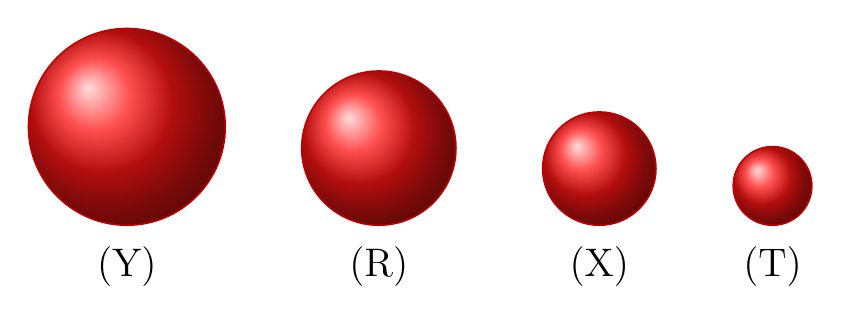
\begin{tikzpicture}
  % Định nghĩa phong cách quả cầu 3D với hiệu ứng bóng đổ và độ chuyển màu tinh xảo
  % Các nguyên tử Y, R, X, T nằm trên cùng một chu kì với bán kính giảm dần:
  % r_Y (1.25cm) > r_R (0.98cm) > r_X (0.72cm) > r_T (0.50cm)
  % Tất cả các quả cầu đều đặt tiếp xúc trên cùng một đường đáy (baseline y = 0)
  
  % --- Quả cầu (Y) ---
  \shadedraw[shading=ball, ball color=red!92!white, draw=red!75!black, line width=0.55pt] 
    (1.4, 1.25) circle (1.25);
  \node[below, font=\fontsize{14}{17}\selectfont] at (1.4, -0.15) {(Y)};

  % --- Quả cầu (R) ---
  \shadedraw[shading=ball, ball color=red!92!white, draw=red!75!black, line width=0.55pt] 
    (4.6, 0.98) circle (0.98);
  \node[below, font=\fontsize{14}{17}\selectfont] at (4.6, -0.15) {(R)};

  % --- Quả cầu (X) ---
  \shadedraw[shading=ball, ball color=red!92!white, draw=red!75!black, line width=0.55pt] 
    (7.4, 0.72) circle (0.72);
  \node[below, font=\fontsize{14}{17}\selectfont] at (7.4, -0.15) {(X)};

  % --- Quả cầu (T) ---
  \shadedraw[shading=ball, ball color=red!92!white, draw=red!75!black, line width=0.55pt] 
    (9.6, 0.50) circle (0.50);
  \node[below, font=\fontsize{14}{17}\selectfont] at (9.6, -0.15) {(T)};

\end{tikzpicture}
\end{document}
